
% This include all the settings that we should use for the document
\newcommand{\PDFTitle}{Using the DESim Application \\ with \hdlName~Designs}
\newcommand{\commonPath}{../../../Tutorials/Common}
\input{\commonPath/Docs/defaulttext.tex}
\input{\commonPath/Docs/preamble.tex}

%%%%%%%%%%%%%%%%%%%%%%%%%
% Add title
\newcommand{\doctitle}{Using the DESim Application \\ with \hdlName~Designs}
\newcommand{\dochead}{Using the DESim Application \\ with \hdlName~Designs}
% Usually no need to change these two lines
\title{\fontfamily{phv}\selectfont{\doctitle} }
\chead{ \small{\textsc{\bfseries \dochead} } }
% Customizations
\newenvironment{ctabbing}%
{\begin{center}\begin{minipage}{\textwidth}\begin{tabbing}}
{\end{tabbing}\end{minipage}\end{center}}

%%%%%%%%%%%%%%%%%%%%%%%%%
% Allows multiple figures per page

\renewcommand\floatpagefraction{.9}
\renewcommand\topfraction{.9}
\renewcommand\bottomfraction{.9}
\renewcommand\textfraction{.1}   
\setcounter{totalnumber}{50}
\setcounter{topnumber}{50}
\setcounter{bottomnumber}{50}
\raggedbottom

\definecolor{AppleGreen}{rgb}{0.55, 0.71, 0.0}
\newcommand{\green}[1]{{\color{AppleGreen}\sf{#1}}}

%%%%%%%%%%%%%%%%%%
%%% DOCUMENT START
\begin{document}
\begin{table}
    \centering
    \begin{tabular}{p{5cm}p{4cm}}
        \hspace{-3cm}
        &
        \raisebox{1\height}{\parbox[h]{0.5\textwidth}{\Large\fontfamily{phv}\selectfont{\textsf{\doctitle}}}}
    \end{tabular}
    \label{tab:logo}
\end{table}

\colorbox[rgb]{0,0.384,0.816}{\parbox[h]{\textwidth}{\color{white}\textsf{\textit{\textBar}}}}

\thispagestyle{plain}
 
\section{Introduction}

This tutorial introduces the {\it DESim} application, which you can use to simulate 
circuits specified with \hdlName~code. The {\it DESim} application provides a 
{\it graphical user interface} (GUI) that represents some of the features of a {\it DE1-SoC}
board. This GUI serves as a ``front end'' for either the {\it ModelSim} or {\it Questa} simulation 
software. Using the {\it DESim} GUI you can invoke both the software's {\it HDL compiler} and 
{\it simulator}. Inputs to the simulator can be provided by clicking on features in the
{\it DESim} GUI, which also shows results produced by the simulator on displays that look
like the ones on a DE1-SoC board.

{\bf Contents:}
\vspace{-1em}
\begin{itemize}
\item Getting Started with {\it DESim}
\item Compiling and Simulating {\it DESim} Sample Projects
\item Simulating a Circuit that Includes a Memory Module
\item Making a {\it DESim} Project
\item Troubleshooting Problems with the {\it DESim} Application
\end{itemize}

{\bf Requirements:}
\vspace{-1em}
\begin{itemize}
	\item A good working knowledge of \hdlName~hardware description language (HDL).
\item A computer running Microsoft\textsuperscript{\textregistered} Windows\textsuperscript{\textregistered} (version 10 is recommended) 
	or Ubuntu Linux.
\item A computer running {\it ModelSim-Intel FPGA} edition software or {\it Questa-Intel FPGA} edition software
\begin{itemize}
	\item If using the {\it ModelSim-Intel FPGA Starter} edition software, version 10.5b is required. It is
		part of the {\it Quartus Prime} suite of CAD tools, versions 18.0, 18.1, 19.0 and 19.1, which are
		provided by Intel\textsuperscript{\textregistered} Corporation.
	\item If using the {\it Questa-Intel FPGA Starter} edition software, version 2021.2 is required. It is
		part of the {\it Quartus Prime} suite of CAD tools, version 21.1, which is
		provided by Intel\textsuperscript{\textregistered} Corporation.
\end{itemize}
\item You should know how to use the simulation software to simulate HDL code using a {\it testbench}. 
	This material is presented in the tutorials: 
		{\it Using ModelSim with Testbenches} and 
		{\it Using Questa with Testbenches}, available from
		\href{https://www.fpgacademy.org/tutorials.html}{FPGAcademy.org}.
%		{\it Using the ModelSim-Intel FPGA Simulator with Verilog/VHDL Testbenches} and 
%		{\it Using the Questa-Intel FPGA Simulator with Verilog/VHDL Testbenches}, available from
%		\href{https://www.fpgacademy.org/tutorials.html}{FPGAcademy.org}.
\item The {\it DESim} application. Instructions for downloading and installing the {\it DESim} 
application are available in the document {\it DESim Installation Guide}, available from
\url{https://github.com/fpgacademy/DESim/releases}.
\end{itemize}

\newpage

\section{Getting Started}
Start the {\it DESim} program to reach the graphical user interface (GUI) shown in 
Figure~\ref{fig:gui}. You should see the message ``\green{The server is running...}'' at 
the top of the {\it message pane} in the GUI. If you do not see this message, but instead 
you see a message \red{Server setup failed}, then the {\it DESim} software is not working
properly and should be closed. In this case, see the troubleshooting section at the end
of this document.

On the right-hand side of Figure~\ref{fig:gui}, the \texttt{LEDs} represent the 
red lights \red{\texttt{LEDR}$_{9-0}$} that are provided on a DE1-SoC board. The
\texttt{Switches} correspond to the board's \blue{\texttt{SW$_{9-0}$}} slide switches, the 
\texttt{Push Buttons} to \blue{\texttt{KEY$_{3-0}$}}, and the \texttt{Seven-segment
Displays} to \red{\texttt{HEX5}}, \red{\texttt{HEX4}}, $\cdots$, \red{\texttt{HEX0}}.
There are also some additional features in the GUI called \texttt{PS/2 Keyboard}, 
\texttt{Parallel Ports}, and \texttt{VGA Display}. These features of
the {\it DESim} GUI are not described in this document. 

\begin{figure}[h]
	\begin{center}
        \setlength{\fboxsep}{0pt}
        \fbox{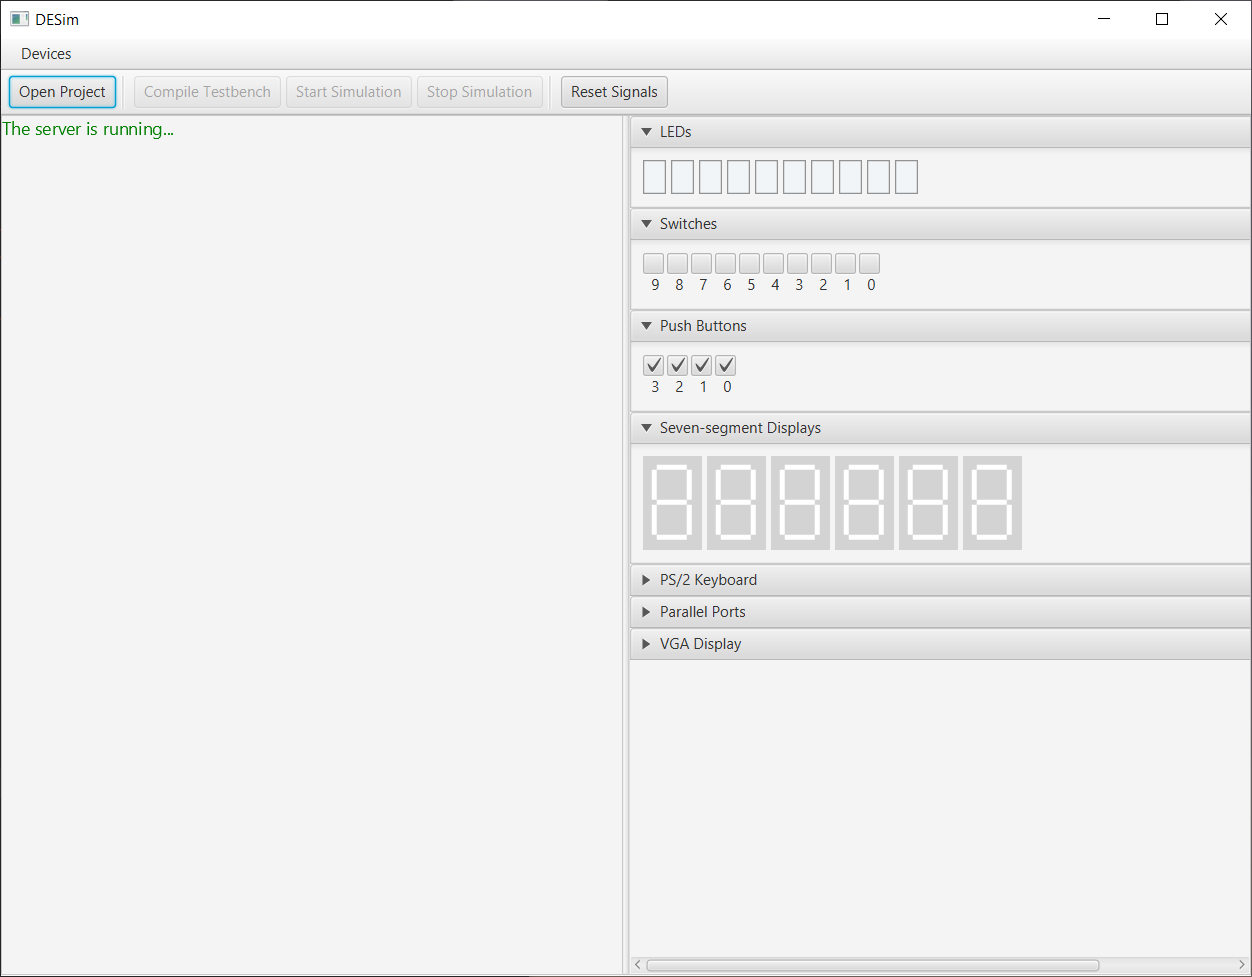
\includegraphics[width = .8\textwidth]{figures/DESim_GUI.png}}
	\end{center}
		  \caption{The {\it DESim} GUI.}
	\label{fig:gui}
\end{figure}

The {\it DESim} tool works in the context of a {\it project}. To introduce the features of the 
{\it DESim} GUI, we will first open an existing project. This example is a multibit adder 
named {\it addern}, which is provided as a {\it demo} project that comes with the {\it DESim}
software. Referring to Figure~\ref{fig:gui}, click on the \texttt{Open Project} command 
to reach the dialogue displayed in Figure~\ref{fig:open_windows} (Windows) or 
Figure~\ref{fig:open_linux} (Linux). As shown in the figures, navigate
to the \texttt{demos} folder, select either \texttt{modelsim/questa} and 
\texttt{systemverilog/verilog/vhdl}, click to select the \texttt{addern} project, and then 
click the \texttt{Select Folder} button in Windows or the \texttt{Open} button in Linux.

\begin{figure}[h]
	\begin{center}
        \setlength{\fboxsep}{0pt}
        \fbox{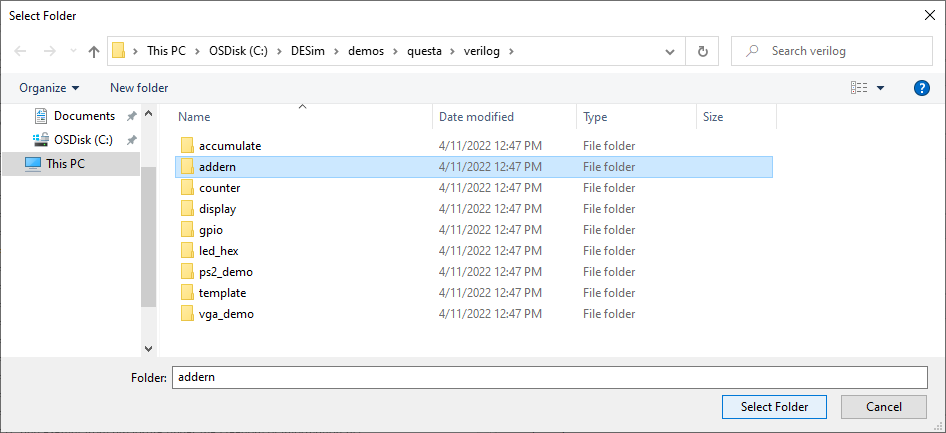
\includegraphics[width = .9\textwidth]{figures/open_addern_windows.png}}
	\end{center}
		  \caption{Opening the {\it addern} project under Windows.}
	\label{fig:open_windows}
\end{figure}

\begin{figure}[h]
	\begin{center}
        \setlength{\fboxsep}{0pt}
        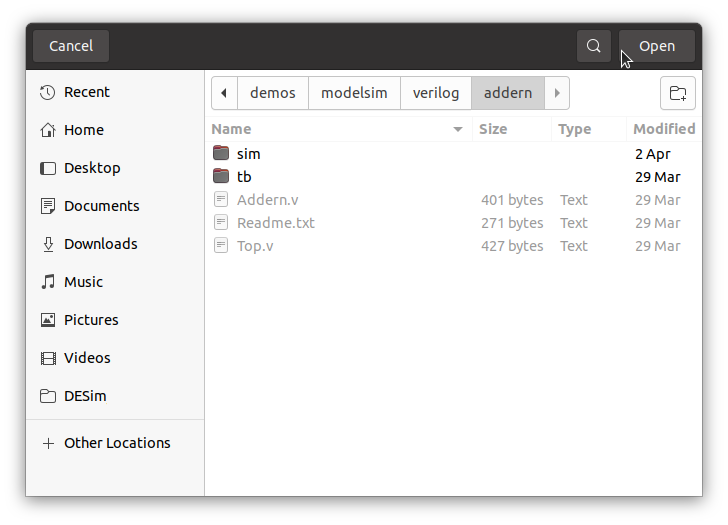
\includegraphics[width = .75\textwidth]{figures/open_addern_linux.png}
	\end{center}
		  \caption{Opening the {\it addern} project under Linux.}
	\label{fig:open_linux}
\end{figure}

\clearpage
\newpage
The {\it addern} project folder, contains the 
folders named \texttt{sim} and \texttt{tb}, as well as the files called {\it Addern.\hdlFileExt}, 
and {\it top.\hdlFileExt}. There is also a {\it Readme.txt} file, but it just provides 
a description of the functionality of this demo and is not really a part of the {\it DESim} project. 

The {\it Addern.\hdlFileExt} file, shown in Figure~\ref{fig:addern}, is the \hdlName~code that will 
be simulated in this part of the tutorial. We will use the {\it DESim} GUI to specify signal 
values for the adder's inputs, {\it Cin}, {\it X}, and {\it Y}, and then display the
simulation results produced for the outputs, {\it Sum} and {\it Cout}, on the \texttt{LEDs}. 
To make connections between the adder's ports and the signals that are associated with the
{\it DESim} GUI, we {\it instantiate} the {\it Addern} \hdlModuleName~in another \hdlName~\hdlModuleName~
called {\it top}. This \hdlModuleName~is defined in the file {\it top.\hdlFileExt}, displayed in 
Figure~\ref{fig:top}. Its ports use the signal names that are appropriate for a
top-level \hdlName~\hdlModuleName~which is intended to be implemented on a DE1-SoC board. These
port names include \texttt{KEY}, \texttt{SW}, and  \texttt{LEDR}.

The {\it Addern} \hdlModuleName~is instantiated in {\it top.\hdlFileExt} by the statement
\ifthenelse{\value{hdlNum}=0}
	{\lstinputlisting[language=Verilog,numbers=none,firstline=12,lastline=12]{../../demos/modelsim/\demos/addern/top.\hdlFileExt}}
	{\lstinputlisting[language=VHDL,numbers=none,firstline=29,lastline=30]{../../demos/addern/top.vhd}}
%\ifnum \value{\hdlNum}=0 {\lstinputlisting[language=Verilog,numbers=none,firstline=12,lastline=12]{../../demos/addern/top.\hdlFileExt}} \else {{\lstinputlisting[language=VHDL,numbers=none,firstline=12,lastline=12]{../../demos/addern/top.\hdlFileExt}}
%\ifnum \value{\hdlNum}=0 {Zero} \else {One}
%\ifthenelse{\value{hdlNum}=0}{Zero}{One}

This statement connects the switch {\it SW}$_9$ to the multibit adder's carry-in, {\it Cin}, 
and it connects {\it SW}$_{3-0}$ and  {\it SW}$_{7-4}$ to the adder's {\it X} and {\it Y} 
data inputs, respectively.  The {\it Sum} output is attached to {\it LEDR}$_{3-0}$, and 
the carry-out, {\it Cout}, is connected to {\it LEDR}$_4$.

\begin{figure}[h]
\begin{center}
\begin{minipage}[h]{15 cm}
\ifthenelse{\value{hdlNum}=0}
	{\lstinputlisting[language=Verilog,numbers=none,firstline=8]{../../demos/modelsim/\demos/addern/addern.\hdlFileExt}}
	{\lstinputlisting[language=VHDL,numbers=none,firstline=9]{../../demos/addern/addern.vhd}}
\end{minipage}
	\caption{The \hdlName~source-code file \texttt{addern.\hdlFileExt}.}
	\label{fig:addern}
\end{center}
\end{figure}

\begin{figure}[h]
\begin{center}
\ifthenelse{\value{hdlNum}=0}
	{\begin{minipage}[h]{15 cm}}
	{\begin{minipage}[h]{18 cm}}
\ifthenelse{\value{hdlNum}=0}
	{\lstinputlisting[language=Verilog,numbers=none,firstline=7]{../../demos/modelsim/\demos/addern/top.\hdlFileExt}}
	{\lstinputlisting[language=VHDL,numbers=none,firstline=8]{../../demos/addern/top.vhd}}
\ifthenelse{\value{hdlNum}=0}
	{\end{minipage}}
	{\end{minipage}}
	\caption{The \hdlName~source-code file \texttt{top.\hdlFileExt}.}
	\label{fig:top}
\end{center}
\end{figure}

To compile the {\it addern} project in the {\it DESim} GUI, click the \texttt{Compile Testbench}
command. This command executes a script called {\it run\_compile}, which is 
found in the \texttt{sim} folder of the {\it addern} project. This script comprises
some {\it ModelSim} commands. The {\it run\_compile.bat} script for Windows is shown below 
(the {\it run\_compile.sh} script for Linux is similar):

\lstinputlisting[language=command.com]{../../demos/modelsim/\demos/addern/sim/run_compile.bat}

The script executes the {\it vlib} command, which is part of the {\it ModelSim/Questa} software,
to create a \texttt{work} folder (while first deleting this folder if it already exists).
The script then invokes the simulation software's Verilog compiler, {\it vlog}, twice. The first invocation
of the compiler, \texttt{vlog ../tb/*.v}, compiles the Verilog source code in the {\it addern}
project's \texttt{tb} folder. This folder holds the {\it testbench} for the project, which is
described shortly. If the SystemVerilog or Verilog version of the {\it addern} project was opened, the 
second call to {\it vlog} compiles the source-code of the {\it addern} project, which includes the files 
{\it Addern.v} and {\it top.v} or {\it Addern.sv} and {\it top.sv}. If instead the SystemVerilog or VHDL 
versions of the {\it Addern} project was opened, the call to {\it vcom} compiles the source-code of the 
{\it Addern} project, which includes the files {\it Addern.vhd} and {\it top.vhd}. Any messages produced 
while executing the {\it run\_compile} script are displayed inside the message pane in the {\it DESim} 
GUI, as illustrated in Figure~\ref{fig:compile}.

\begin{figure}[h]
	\begin{center}
        \setlength{\fboxsep}{0pt}
        \fbox{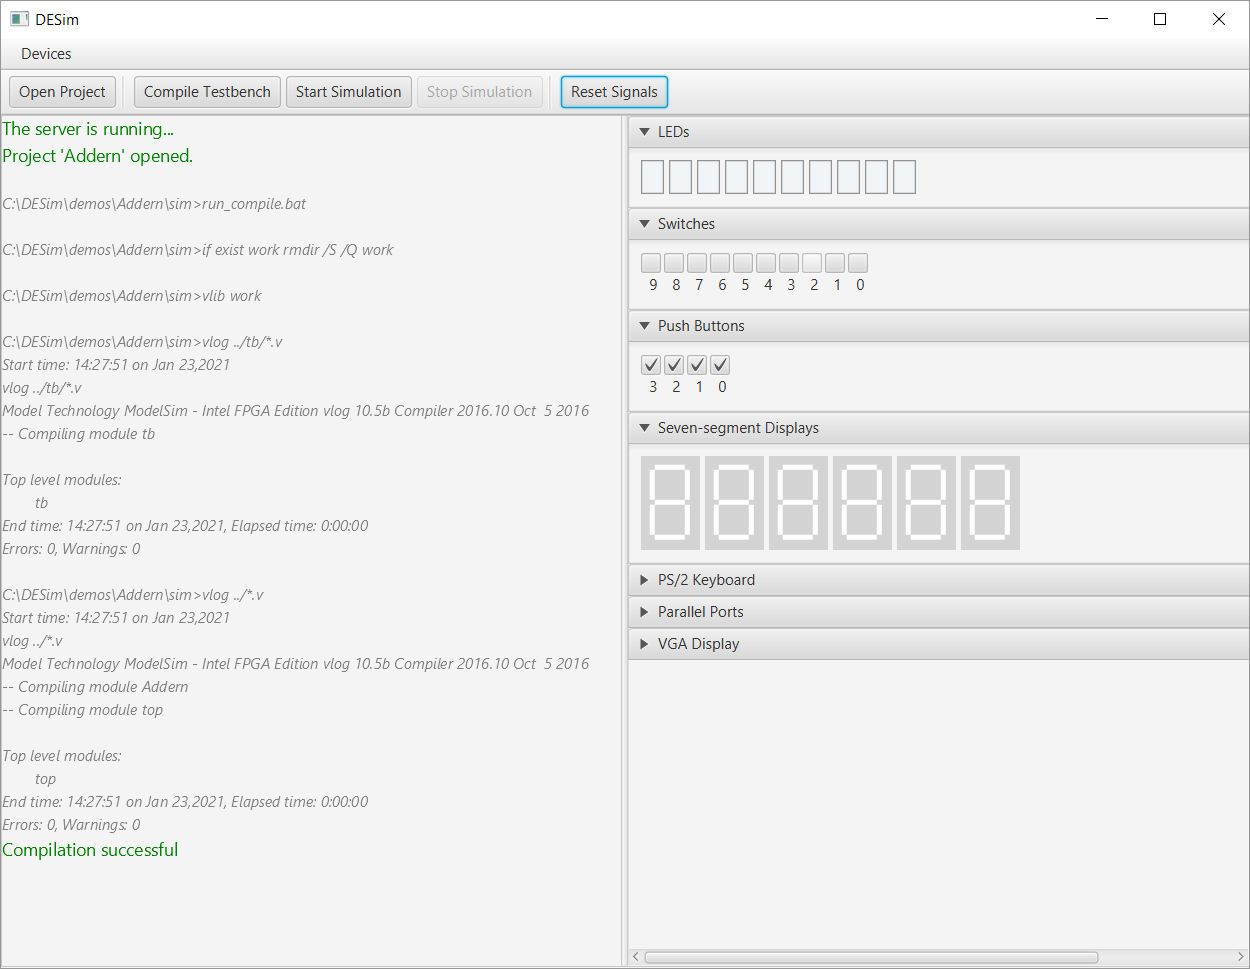
\includegraphics[width = \textwidth]{figures/run_compile.png}}
	\end{center}
          \caption{Messages produced by executing the {\it run\_compile} script.}
	\label{fig:compile}
\end{figure}

\newpage
The testbench file for the {\it addern} project that is compiled by the command 
\texttt{vlog ../tb/*.v} is called {\it tb.v}, and is displayed in Figure~\ref{fig:tb}. 
It is not necessary to modify (or even examine) much of this code to use the {\it
DESim} software, but we describe some of the code here for completeness.
The testbench code in the figure has a general structure that 
allows it to be used to simulate different HDL code
that might be used in various {\it DESim} projects. Hence, not
all of the code in the testbench is needed for the {\it addern} project.  The first line 
declares the testbench \hdlModuleName, which is named {\it tb}. 
The next several lines in the code declare some signals that are used in the testbench. 
The statement

\lstinputlisting[language=Verilog,numbers=none,firstline=29,lastline=30]{../../demos/modelsim/verilog/addern/tb/tb.v}

is unique to the {\it DESim} program. It makes use of a special feature of the
{\it ModelSim/Questa} software that allows communication with a 
{\it custom software function}. In this case, the custom function is part of the {\it DESim} 
software and is called {\it sim\_fpga}. This function is stored in a file named {\it simfpga.vpi}, 
which has to be included in the \texttt{sim} folder of each {\it DESim} project. The {\it DESim} 
GUI sends/receives signal values to/from the simulation software via the {\it sim\_fpga} function. 
This capability is known as the {\it Verilog Procedural Interface} (VPI). 

\begin{figure}[H]
\begin{center}
\begin{minipage}[t]{16.5 cm}
%	\lstinputlisting[language=Verilog,numbers=none,firstline=8]{../../demos/addern/tb/tb.v}
	\lstinputlisting[language=Verilog,numbers=none,linerange={9-31, 34-37,
    46}]{../../demos/modelsim/verilog/addern/tb/tb.v}
\end{minipage}
	\caption{The testbench file, {\it tb.v}, for the {\it addern} project.}
	\label{fig:tb}
\end{center}
\end{figure}

The second last line in the testbench code instantiates the 
{\it design under test} (DUT), which is the \hdlName~\hdlModuleName~named {\it top} shown in 
Figure~\ref{fig:top}. To execute the testbench using the simulator, click on the
\texttt{Start Simulation} command in the {\it DESim} GUI. This command executes a script 
called {\it run\_sim}, which is found in the \texttt{sim} folder of the 
{\it addern} project. This script runs {\it vsim}, the {\it ModelSim/Questa} Verilog
simulator, using one of the commands:

\lstinputlisting[language=command.com]{../../demos/modelsim/verilog/addern/sim/run_sim.bat}

The \texttt{-pli} argument for the {\it vsim} program instructs it to link to the
{\it sim\_fpga} software function that has been (previously) compiled into the 
{\it simpfga.vpi} file. The \texttt{-L} arguments include some simulation libraries for
Intel FPGAs that may be needed by the simulator. The \texttt{-t} argument specifies
the simulator time resolution. Finally, the remaining arguments 
run the simulation for the top-level \hdlModuleName, which is {\it tb}. Any messages 
produced while executing the {\it run\_sim} script are displayed inside the message pane in
the {\it DESim} GUI, as depicted in Figure~\ref{fig:sim}.

As mentioned previously, the {\it addern} project includes a {\it Readme.txt} file that
documents its usage. This file is displayed in Figure~\ref{fig:readme}. You can follow
its instructions to see how the switches and lights are used for the project (of course, 
you can also find this information by looking at the \hdlName~source code). An example
simulation result is illustrated in Figure~\ref{fig:sim}. It corresponds to {\it Cin} $= 1$,
$X = (0110)_2 = (6)_{10}$, and $Y = (1010)_2 = (10)_{10}$. The result of the addition is
$(10001)_2 = (17)_{10}$ ({\it Cout} $= 1$, with {\it Sum} $= (0001)_2$), which is displayed on 
the \texttt{LEDs}.  Try different settings for the
\texttt{SW} switches and observe the results displayed on the \texttt{LEDs}.

\begin{figure}[h]
	\begin{center}
        \setlength{\fboxsep}{0pt}
        \fbox{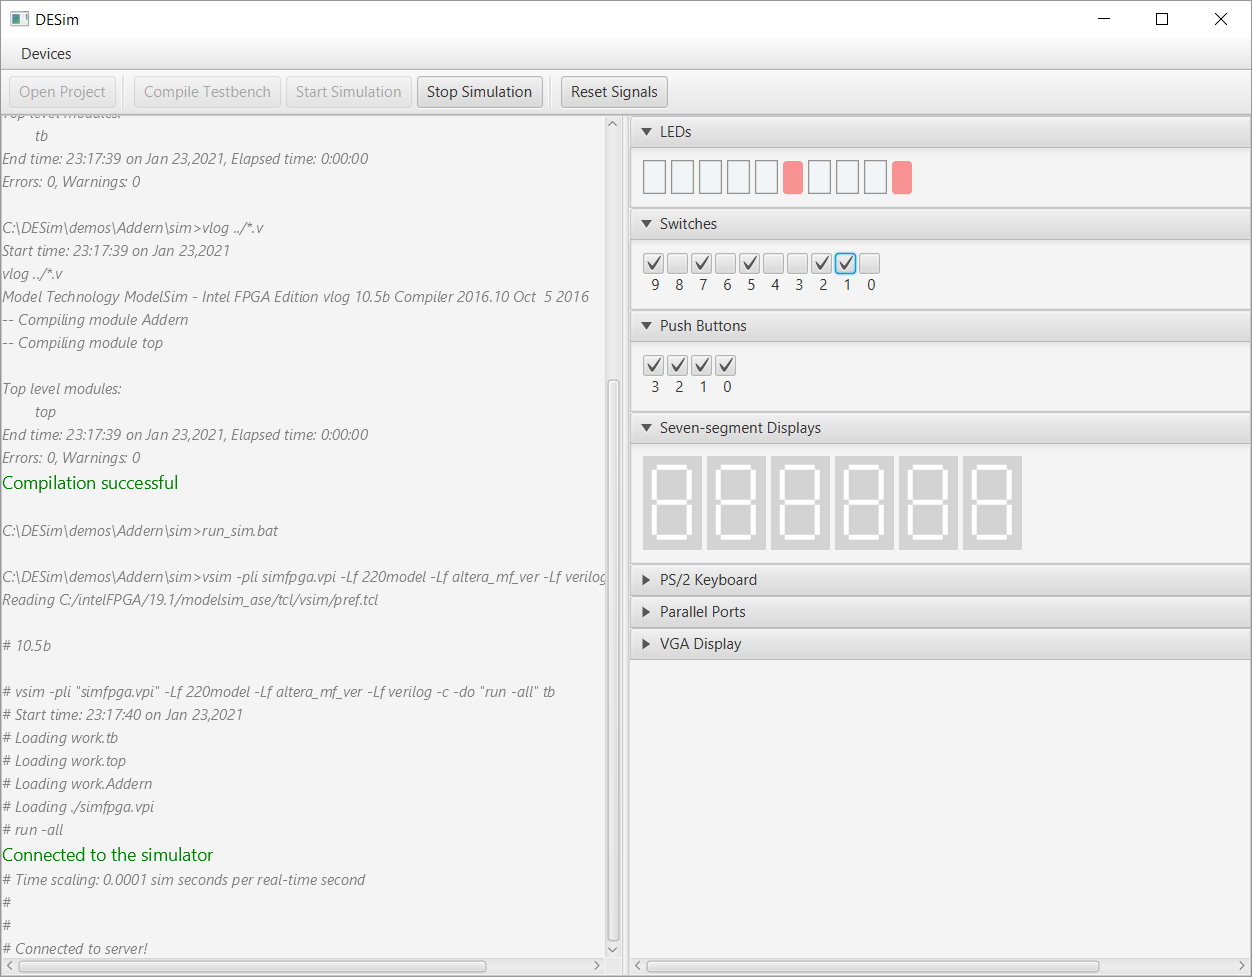
\includegraphics[width = \textwidth]{figures/run_simulation.png}}
	\end{center}
          \caption{Messages produced by executing the {\it run\_sim.} script.}
	\label{fig:sim}
\end{figure}

\begin{figure}[H]
\begin{center}
\begin{minipage}[t]{15 cm}
	\lstinputlisting[numbers=none]{../../demos/modelsim/verilog/addern/Readme.txt}
\end{minipage}
    \caption{The {\it Readme.txt} file for the {\it addern} project.}
	\label{fig:readme}
\end{center}
\end{figure}

We have now finished discussing the {\it addern} sample project.

\section{Simulating a Sequential Circuit}

Another {\it DESim} sample project called {\it counter} is included in the {\it DESim}
\texttt{demos} folder. Use the \texttt{Open Project} command in the {\it DESim} GUI to open this
project. The contents of the file-system folder for this project look the same as for the 
{\it addern} project, except that there is a \hdlName~source-code file named {\it Counter.\hdlFileExt}. 
Figure~\ref{fig:counter} shows the contents of the {\it Counter.\hdlFileExt} file. It represents a 
24-bit counter with synchronous reset. The {\it LEDR} port name corresponds to the red LEDs
on the DE1-SoC board. Since {\it LEDR} port is a 10-bit signal and the 
counter has 24 bits, only a subset of the counter outputs (the most-significant ones) are 
connected to {\it LEDR}.

\begin{figure}[h]
\begin{center}
\begin{minipage}[h]{15 cm}
\ifthenelse{\value{hdlNum}=0}
	{\lstinputlisting[language=Verilog,numbers=none,firstline=10]{../../demos/modelsim/\demos/counter/Counter.\hdlFileExt}}
	{\lstinputlisting[language=VHDL,numbers=none,firstline=11]{../../demos/counter/Counter.vhd}}
\end{minipage}
	\caption{The \hdlName~code for the 24-bit counter.}
	\label{fig:counter}
\end{center}
\end{figure}

As described for the {\it addern} project, the {\it Counter} \hdlModuleName~is {\it instantiated}
in another \hdlName~\hdlModuleName~called {\it top}. This \hdlModuleName~is displayed in 
Figure~\ref{fig:counter_top}. It is similar to the one from Figure~\ref{fig:top}, except that 
it includes a clock, {\it CLOCK\_50}, input port and instantiates the {\it Counter} \hdlModuleName.
The port names for this \hdlModuleName, correspond to the signal names on the DE1-SoC board, 
with {\it CLOCK\_50} for the clock signal, and {\it KEY}$_0$ being used for reset.

\begin{figure}[h]
\begin{center}
\begin{minipage}[h]{15 cm}
\ifthenelse{\value{hdlNum}=0}
	{\lstinputlisting[language=Verilog,numbers=none,firstline=7]{../../demos/modelsim/\demos/counter/Top.\hdlFileExt}}
	{\lstinputlisting[language=VHDL,numbers=none,firstline=8]{../../demos/counter/Top.vhd}}
\end{minipage}
	\caption{The {\it top} \hdlModuleName~for the {\it counter} project.}
	\label{fig:counter_top}
\end{center}
\end{figure}

To compile the {\it counter} project, in the {\it DESim} GUI click the \texttt{Compile Testbench}
command. This command executes the {\it run\_compile} script, which
is found in the \texttt{sim} folder of the {\it counter} project. This script 
is identical to the one described earlier for the {\it addern} project. 
The testbench file that is compiled by {\it run\_compile} for the {\it counter} project is  
found in its \texttt{tb} folder. This testbench, {\it tb.v}, is similar to the one shown 
in Figure~\ref{fig:tb}, except that it includes a \texttt{CLOCK\_50} signal in the DUT instantiation.

To execute the testbench for the {\it counter} project, click on the
\texttt{Start Simulation} command in the {\it DESim} GUI. This command executes the
{\it run\_sim} script. It is identical the one described for the 
{\it addern} project and runs the {\it vsim} simulator.

The {\it Readme.txt} file for the {\it counter} project specifies:

\lstset{language=make,numbers=none,escapechar=|}
\begin{lstlisting}[]
To use this demo, reset the circuit by pressing and releasing KEY[0].
\end{lstlisting}

In the {\it DESim} GUI, when the \texttt{Push Buttons} have a check mark shown, they are set to the
value 1. To reset the counter circuit, click \texttt{KEY}$_0$ once to {\it press} this button
(this action sets the corresponding signal for this button to 0), and then click it again
to {\it release} the button. The 24-bit counter will start to operate and the ten
most-significant counter outputs will be displayed on the \texttt{LEDs}. A screen-shot of
the {\it DESim} GUI while simulating the {\it counter} project is shown in 
Figure~\ref{fig:sim2}.

\begin{figure}[h]
	\begin{center}
        \setlength{\fboxsep}{0pt}
        \fbox{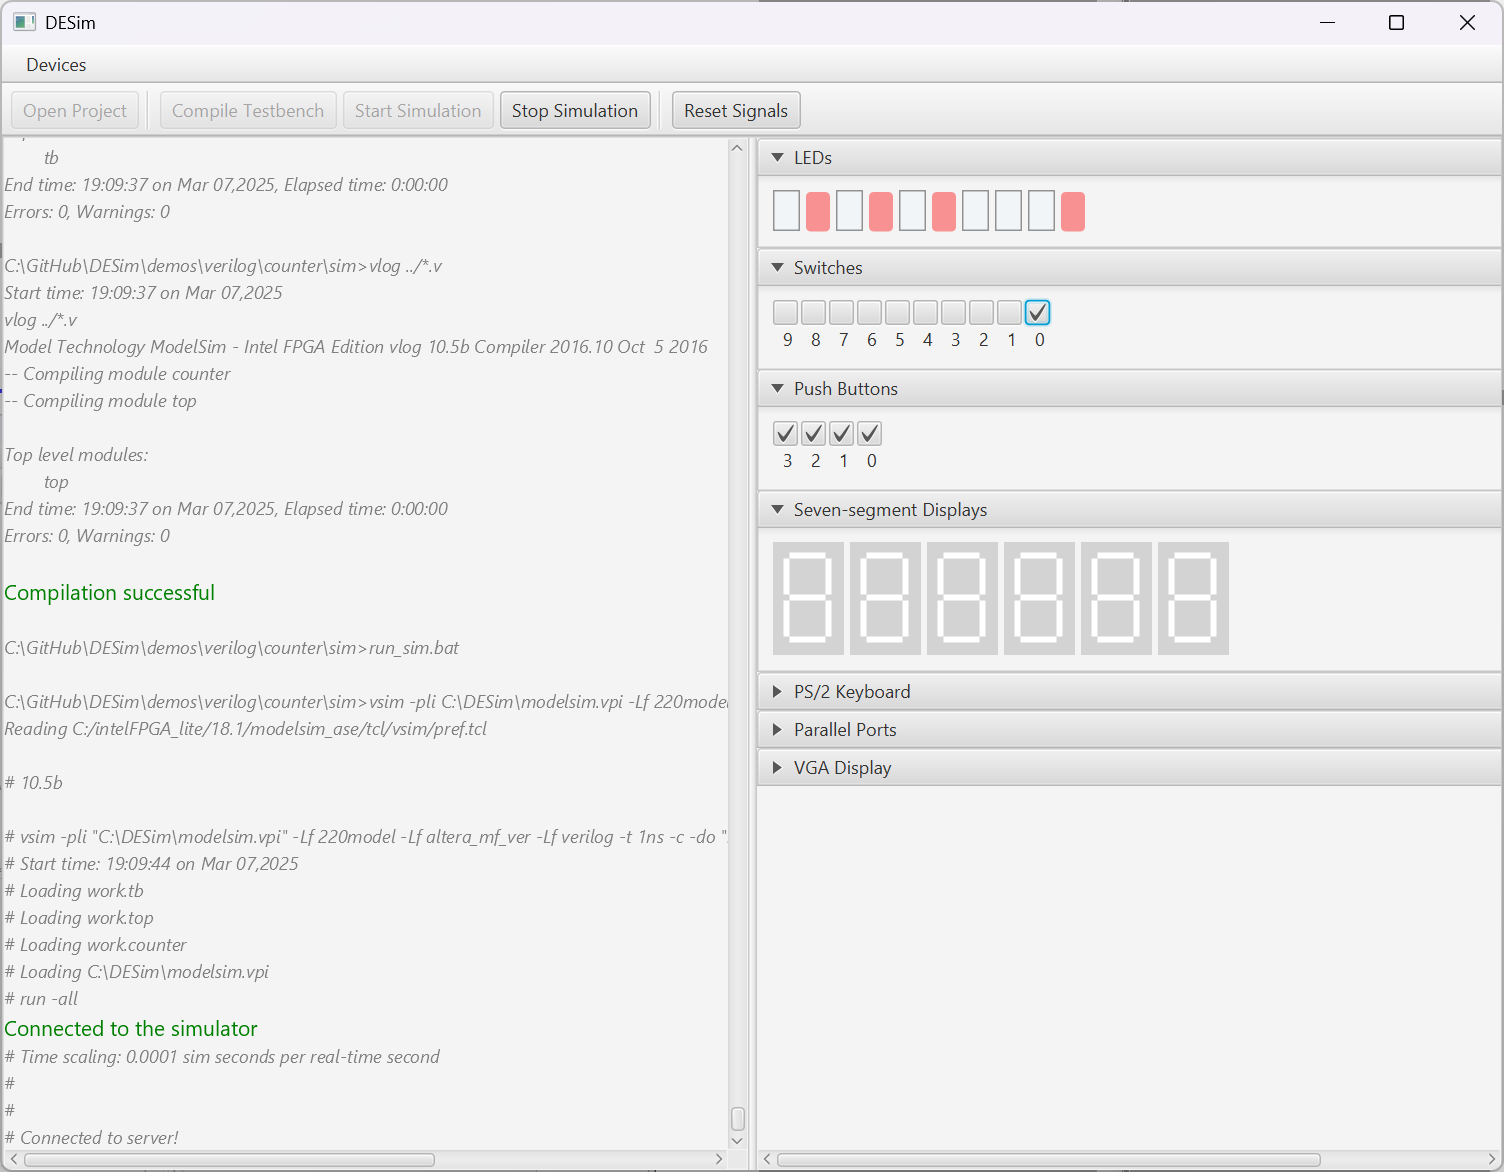
\includegraphics[width = \textwidth]{figures/run_simulation2.png}}
	\end{center}
          \caption{Simulating the {\it counter} project.}
	\label{fig:sim2}
\end{figure}

%\newpage
\section{Simulating a Circuit that Includes a Memory Module}

The {\it DESim} \texttt{demos} folder includes a project called {\it display}. It shows how 
to instantiate a memory \hdlModuleName, and how to initialize the stored contents of 
the memory in a {\it DESim} simulation.  Use the \texttt{Open Project} command to open this
example project. The contents of the file-system folder for this project look similar to the 
previous ones, but there are two extra files: {\it inst\_mem.v} and {\it inst\_mem.mif}. These 
files are used for the memory \hdlModuleName~in the circuit, which is described shortly.

Figure~\ref{fig:display} shows the \hdlName~code for {\it Display.\hdlFileExt}, which 
has ports named {\it CLOCK}, {\it RESETn}, {\it HEX0}, and {\it LEDR}.
Figure~\ref{fig:memory}$a$ gives a logic circuit that corresponds to the code in 
Figure~\ref{fig:display}. The circuit contains a counter that is used to read the 
contents of successive locations in a memory. This memory provides codes in ASCII format 
for some upper- and lower-case letters, which are provided as inputs to a decoder \hdlModuleName. 
The counter and memory modules have a common clock signal, and the counter has a
synchronous clear input. Each successive clock cycle advances the counter and reads 
a new ASCII code from the memory. Since the counter is three-bits wide, only the first 
eight locations in the memory are read (the upper two address bits on the memory are set
to 00), and they provide the ASCII codes for letters A, b, C, d, E, F, g, and h. The 
decoder produces an appropriate bit-pattern to render each letter on a seven-segment display.

The memory used in the logic circuit is depicted in part $b$ of Figure~\ref{fig:memory}. It
is a $32 \times 8$ synchronous read-only memory (ROM), which has a register for holding 
address values. The memory is specified in the Verilog file {\it inst\_mem.v}, and it is 
initialized with the contents of the file {\it inst\_mem.mif},
which is illustrated in Figure~\ref{fig:mif}. This file contains the ASCII codes for the 
eight letters displayed by the circuit.

\begin{figure}[h]
\begin{center}
\begin{minipage}[h]{15 cm}
\ifthenelse{\value{hdlNum}=0}
	{\lstinputlisting[language=Verilog,numbers=none,firstline=9]{../../demos/modelsim/\demos/display/Display.\hdlFileExt}}
	{\lstinputlisting[language=VHDL,numbers=none,linerange={10-28, 43-68}]{../../demos/display/Display.vhd}}
\end{minipage}
	\caption{The \hdlName~code for the {\it display} project.}
	\label{fig:display}
\end{center}
\end{figure}

\ifthenelse{\value{hdlNum}=0}{}{
\begin{figure}[h]
\begin{center}
\begin{minipage}[h]{15 cm}
	\lstinputlisting[language=VHDL,numbers=none,firstline=75]{../../demos/display/Display.vhd}
\end{minipage}
	\caption{The \hdlName~code for the {\it display} project (Part b).}
	\label{fig:displayb}
\end{center}
\end{figure}
}

\begin{figure}[t]
	\begin{center}
		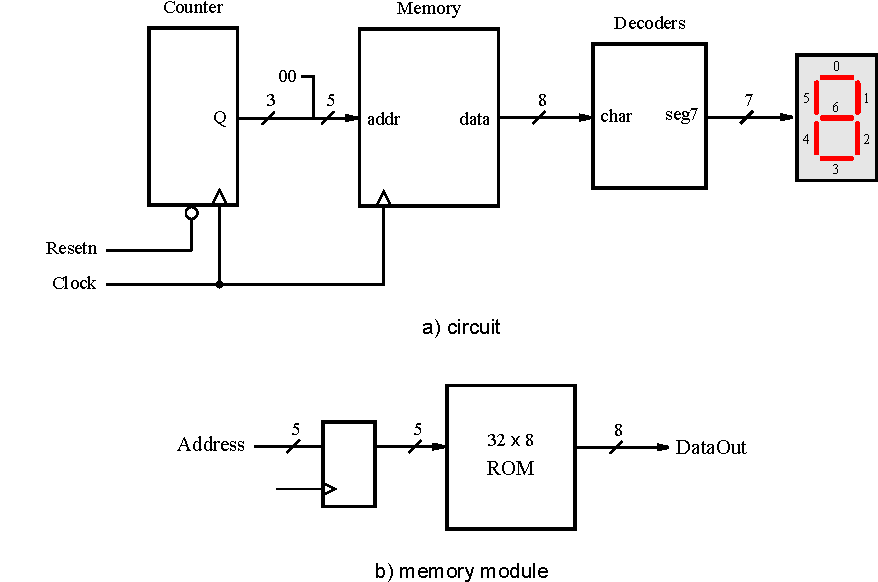
\includegraphics[scale = 1.0]{figures/figdisplay.pdf}
	\end{center}
          \caption{A circuit that represents the {\it display} project.}
	\label{fig:memory}
\end{figure}

\begin{figure}[bh!]
\begin{center}
\begin{minipage}[t]{12.5 cm}
\begin{tabbing}
DEPTH = 32;\\
WIDTH = 8;\\
ADDRESS\_RADIX = HEX;\\
DATA\_RADIX = DEC;\\
CONTENT\\
BEGIN\\
BEGI\=00X\=: \=104;XXXX\=\% A \=\% \kill
\>00 \>: \>65;    \>\% A \>\%\\
\>01 \>: \>98;    \>\% b \>\%\\
\>02 \>: \>67;    \>\% C \>\%\\
\>03 \>: \>100;   \>\% d \>\%\\
\>04 \>: \>69;    \>\% E \>\%\\
\>05 \>: \>70;    \>\% F \>\%\\
\>06 \>: \>103;   \>\% g \>\%\\
\>07 \>: \>104;   \>\% h \>\%\\
END;
\end{tabbing}
\end{minipage}
\end{center}
    \caption{The {\it inst\_mem.mif} memory initialization file.}
\label{fig:mif}
\end{figure}

\clearpage
\newpage
\noindent
To compile the {\it display} project, in the {\it DESim} GUI click the \texttt{Compile Testbench}
command. This command executes the project's {\it run\_compile} script, which
is in its \texttt{sim} folder. This {\it Windows} batch script is shown below (the {\it Linux}
shell script is similar):

\lstinputlisting[language=command.com]{../../demos/modelsim/\demos/display/sim/run_compile.bat}

Lines 1 to 3 are used to copy the memory initialization file,
{\it inst\_mem.mif}, from the \texttt{display} project folder into the \texttt{sim}
folder. This is done for two reasons: 1. {\it ModelSim/Questa} require the file to be in the
\texttt{sim} folder to properly initialize the memory module during a simulation, and 2. 
if the file is changed in the \texttt{display} folder, then the latest version of the file 
will always be used when starting a simulation. The rest of the script, which compiles the 
HDL code, is the same as for the previously-described {\it DESim} projects, except of the 
{\it vlog ../*.v} line. This line is now always executed, as the memory initialization module 
is written in Verilog, even if the SystemVerilog or VHDL versions were chosen.

The testbench file {\it tb.v} that is compiled by {\it run\_compile} script for the {\it display}
project is similar to the one used for the {\it addern} project, shown in Figure~\ref{fig:tb}. The
one difference, is the inclusion of the {\it CLOCK\_50} signal in the \texttt{DUT} instantiation.
To execute the testbench for the {\it display} project, click on 
\texttt{Start Simulation}. Its {\it run\_sim} script is the same as the 
ones used for the {\it addern} and {\it counter} projects.

The {\it Readme.txt} file for the {\it display} project is shown in Figure~\ref{fig:readme2}.
You can follow its instructions to read successive locations out of the memory and
display the corresponding characters on \texttt{HEX0}. An example simulation output after
first resetting the circuit and then creating a few clock cycles using \texttt{KEY[0]}
is illustrated in Figure~\ref{fig:sim3}.

\lstset{language=make,escapechar=|}
\begin{figure}[h]
\begin{center}
\begin{minipage}[t]{12.5 cm}
	\lstinputlisting{../../demos/modelsim/\demos/display/Readme.txt}
\end{minipage}
    \caption{The {\it Readme.txt} file for the {\it display} project.}
\label{fig:readme2}
\end{center}
\end{figure}

\begin{figure}[t]
	\begin{center}
        \setlength{\fboxsep}{0pt}
        \fbox{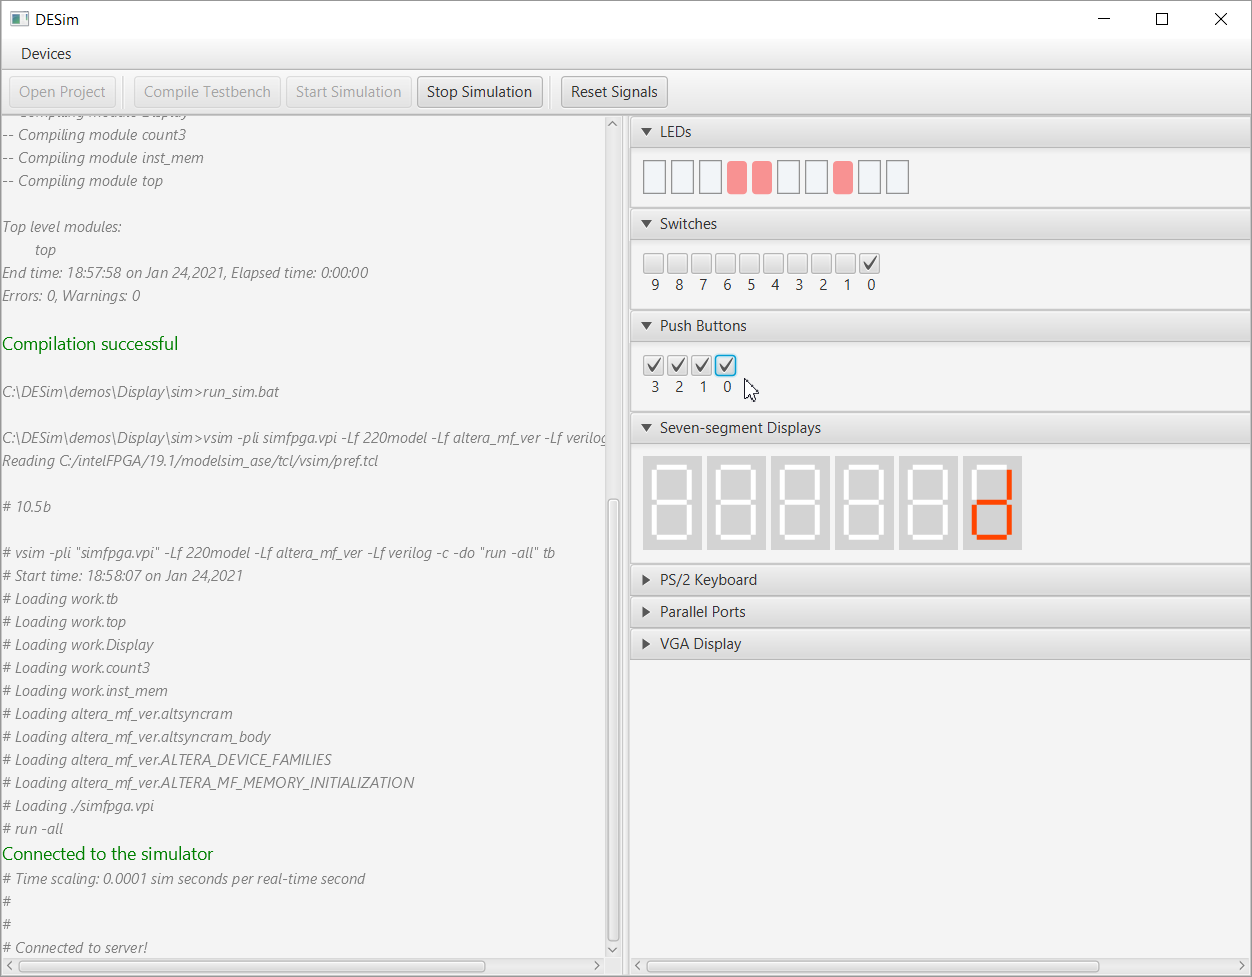
\includegraphics[width = \textwidth]{figures/run_simulation3.png}}
	\end{center}
          \caption{Simulating the {\it display} project.}
	\label{fig:sim3}
\end{figure}

\section{Setting up a {\it DESim} Project}

An easy way to set up your own {\it DESim} project is to use one of the example projects in
the {\it DESim} \texttt{demos} folder as a starting point. You should choose a specific 
\texttt{demo} project according to its features. 
For example, if your design project includes a memory module, then you might choose to start 
with a copy of the {\it display} project. But if you do not require a memory module, then 
you could start with a copy of one of the other projects. Also, you should start
with a project that has the ports that you need in its ``top'' \hdlModuleName~that is instantiated by
its testbench. The various projects included in the \texttt{demos} folder 
may have different top-level ports. 

Once you choose a project from the \texttt{demos} folder as a starting point, you should
copy its folder contents into a new folder on your computer. For example, you might make a copy of
\texttt{demos$\backslash$questa$\backslash$verilog$\backslash$display} and call the new folder 
\texttt{my\_folder}. Then, in
\texttt{my\_folder} you would replace the file {\it Display.\hdlFileExt} with your own source-code 
file, say {\it my\_source.\hdlFileExt}. Next, you would edit the file {\it top.\hdlFileExt} in 
\texttt{my\_folder} and change it to instantiate your \hdlName~\hdlModuleName, say {\it my\_\hdlModuleName} (which 
would be in the file {\it my\_source.\hdlFileExt}). You would connect 
the signals in {\it top.\hdlFileExt}, such as \texttt{CLOCK\_50}, \texttt{KEY}, and so on, 
as needed to the ports of {\it my\_\hdlModuleName}. If some of the ports that you require for 
{\it my\_\hdlModuleName} aren't available in the {\it top} \hdlModuleName, then you should instead use
a different sample project from the \texttt{demos} folder that has the required 
ports in its {\it top} \hdlModuleName.  

You should not need to make any changes to the files in the \texttt{sim} or \texttt{tb} folder 
for your new project in \texttt{my\_folder}. You can now open your new project in the
{\it DESim} software and proceed to compile/simulate your code. 

\newpage
\section{Troubleshooting Problems with the {\it DESim} Software}

This section discusses some potential issues that could be encountered while using the
{\it DESim} software, and provides suggested solutions.

\begin{enumerate}
\item Upon starting the {\it DESim} software you should see the message 
\green{The server is running...}'' at the top of the {\it message pane} in the GUI. If you do 
not see this message, but instead see a message \red{Server setup failed}, then 
the {\it DESim} software is not working properly and should be closed. One
reason why this would occur is if you have executed a {\it second}
instance of the {\it DESim} program. The {\it DESim} software cannot be
executed more than once concurrently on your computer. 

\item If you click on the \texttt{Compile Project} command in the {\it DESim} GUI, it is
possible to see an error message such as 
\red{`vlib' is not recognized as an internal or external command'}. This error means that
{\it DESim} attempted to execute the {\it vlib} program, which is part of the 
{\it ModelSim/Questa} software, but the program was not found by the
operating system. This error will occur if the {\it ModelSim/Questa} software is not installed 
on the computer, or if it is installed but cannot be be located. There are two ways to fix the
latter issue: 1) the\texttt{Path} environment variable can be 
updated to include the location of the {\it ModelSim/Questa} software, or 2) the location of the
{\it ModelSim/Questa} software can be specified within the batch script that starts
the {\it DESim} software. This script is called {\it DESim\_run} and is found
in the file-system folder where {\it DESim} is installed. 

\item Occasionally, when compiling or simulating a project in the {\it DESim} software you may
see a {\it Warning} message which says that {\it ModelSim/Questa} cannot ``unlink'' a file. 
For example, if your {\it DESim} project is stored in the folder
C:$\backslash$DESim$\backslash$demos$\backslash$addern, then this message would report: 

\noindent
\begin{minipage}[h]{18 cm}
\lstset{language=command.com,numbers=none,escapechar=|,moredelim=**[is][\color{RedOrange}]{@}{@}}
\begin{lstlisting}[]
@** Warning: (vlog-31) Unable to unlink file "C:/DESim/demos/addern/sim/work/_lock"@
\end{lstlisting}
\end{minipage}

This problem occurs for unknown reasons and is caused by an issue with the
{\it ModelSim/Questa} software (it happens when directly using the ModelSim/Questa GUI
also, and not only when using the {\it DESim} tool). If the ``unlink'' issue
persists (sometime it gets resolved automatically), then a
solution is to browse with \texttt{File Explorer} into the file-system folder  
\texttt{C:$\backslash$DESim$\backslash$demos$\backslash$addern$\backslash$sim$\backslash$work}
and manually {\it delete} the file named {\it \_lock}.

\item If you click on the \texttt{Start Simulation} command in the {\it DESim} GUI,
an error message such as \red{Load of "./simfpga.vpi" failed: Bad DLL Format} might happen.
This error occurs if the {\it ./simfpga.vpi} DLL is not compatible with the installed simulator.
Make sure that you are using the corresponding {\it ./simfpga.vpi} DLL generated for 
{\it ModelSim} when using the {\it ModelSim} simulator, and the one generated for
{\it Questa} when using the {\it Questa} simulator. They can be found in the corresponding
demo directories. If the error is still present, verify that the correct version of the
{\it ModelSim/Questa} software is been used. Refer to the {\it DESim} Installation
Guide for supported versions.
\end{enumerate}

% Copyright and Trademark

\input{\commonPath/Docs/copyright.tex}

\end{document}
